% !TEX encoding = UTF-8
% !TEX TS-program = pdflatex
% !TEX root = ../relazione-finale.tex

%**************************************************************
\pagebreak
\chapter{Svolgimento dello stage}
\label{cap:descrizione-stage}
%**************************************************************

\section{Ambiente di sviluppo}

In questa sezione descrivo le tecnologie e gli strumenti di sviluppo che ho utilizzato per lo sviluppo del progetto, includendo la motivazione per cui ho fatto la scelta.
Nella tabella ~\ref{tab:tecnologie} presento il sommario delle tecnologie e degli strumenti che ho utilizzato per lo sviluppo del prototipo, indicandone:
\begin{itemize}
  \item il nome;
  \item una breve descrizione;
  \item la versione utilizzata o l'intervallo di versioni utilizzate nel caso in cui abbia aggiornato le tecnologie o gli strumenti utilizzati ad una versione successiva;
  \item il grado di conoscenza pregressa in una scala crescente che parte da 0 (esperienza nulla) e che arriva a 5 (esperienza consolidata), abbreviato in "Esp.".
\end{itemize}

\begin{table}[!htbp]
\caption{Tabella con il sommario delle tecnologie e degli strumenti utilizzati}
\label{tab:tecnologie}
\begin{tabularx}{\linewidth}{|c|>{\hsize=1.6\hsize}X|>{\hsize=0.4\hsize}X|c|}
\hline
\textbf{Tecnologia} & \textbf{Descrizione} & \textbf{Versioni} & \textbf{Esp.}\\
\hline
Node.js & Node.js è un'ambiente d'esecuzione utilizzato per l'implementazione di applicazioni server in JavaScript. & v9.2.0, \newline v9.2.1 & 4 \\
\hline
React & React è una libreria per il linguaggio JavaScript il cui scopo è costruire interfacce grafiche. & v16.2.0 & 3 \\
\hline
ECMAScript 2017 & ECMAScript è un linguaggio di programmazione la cui implementazione standard più conosciuta è JavaScript. & 06/2017 & 2 \\
\hline
Jest & Jest è un \emph{framework} per l'implementazione di test per codice JavaScript. & v21.2.1 & 3 \\
\hline
ESLint & ESLint è uno strumento \emph{open source} per l'analisi statica del codice JavaScript prodotto. & v4.12.0, \newline v4.12.1 & 4 \\
\hline
HTML5 & HTML5 è un linguaggio di \emph{markup} per la formattazione e impaginazione delle pagine \emph{web}. & N.D. & 4 \\
\hline
CSS3 & CSS3 è un linguaggio di formattazione delle pagine \emph{web}. & N.D. & 2 \\
\hline
Docker Engine & Docker Engine è la combinazione dell'implementazione della tecnologia di containerizzazione con gli strumenti di gestione del ciclo di vita dei \emph{container}. & v17.09.0, \newline v17.12.0 & 4 \\
\hline
Docker Compose & Docker Compose è lo strumento attraverso cui è possibile coordinare applicazioni eseguite su \emph{container} multipli. & v1.18.0 & 1 \\
\hline
Atom & Atom è un \emph{editor} di testo sviluppato da \gls{GitHub}. & v1.21.2, \newline v1.23.1 & 4 \\
\hline
VS Code & Visual Studio Code è un \emph{editor} di testo sviluppato da \gls{Microsoft}. & v1.18.1, \newline v1.19.1 & 1 \\
\hline
\end{tabularx}
\end{table}

% \subsection{Node.js}
%



% \section{MQTT}
% \label{subsec:mqtt}
%
%
% MQTT mira ad assere una soluzione semplice da implementare, per permettere la maggior copertura di dispositivi possibile.
% MQTT usa messaggistica pub/sub per permettere ai dispositivi di pubblicare nella rete informazioni non predefinite.
% MQTT non richiede amministrazione in quanto cerca di rispondere ad eventi inaspettati in maniera semplice e con maggior buon senso possibile.
% MQTT minimizza il traffico sulla rete introducendo un \gls{overhead} sui dati minimo.
% MQTT si aspetta di lavorare in reti con frequenti interruzioni, utilizzando il meccanismo dell'ultimo testamento.
% MQTT si accorge repentinamente di cambiamenti dello stato della sessione.
% MQTT si aspetta che i \emph{client} abbiano risorse d'elaborazione limitate.
% MQTT mette a disposizione livelli di affidabilità per la trasmissione di informazioni critiche.
% MQTT non fa assunzioni sulla struttura né il contenuto dei dati.

\newpage

%**************************************************************
\section{Analisi dei requisiti}
\label{ar}

Ho iniziato l'Analisi dei requisiti cercando di capire quali funzionalità dovesse offrire il prototipo; per affrontare al meglio la definizione di queste funzionalità, ho esplorato il mercato dei dispositivi IoT esistenti per individuare i limiti del dominio applicativo in cui questi dispositivi si inseriscono.
Ho osservato che una delle caratteristiche desiderabili che il sistema deve offrire riguarda l'identificazione precisa di quali dispositivi sono collegati al sistema; per questo ho vincolato l'accesso dei dispositivi al sistema: per accedervi i dispositivi devono fornire informazioni relative a modello, revisione, produttore e anno di produzione del dispositivo, oltre a un seriale univoco.

Ho inoltre suddiviso i dispositivi in due tipi principali in base alle funzionalità che essi offrono:
\begin{itemize}
	\item sensori;
	\item dispositivi che ho definito "attivi".
\end{itemize}
La funzionalità principale offerta dai sensori è l'invio periodico di informazioni legate a ciò che il sensore misura.
L'invio di informazioni periodiche avviene in automatico, secondo i parametri impostati dal produttore del sensore.

Nella mia analisi delle funzionalità richieste dai dispositivi attivi, ho considerato le seguenti funzionalità:
\begin{itemize}
	\item pubblicazione di una lista degli eventi gestiti dal dispositivo;
	\item generazione di risposte agli eventi esterni;
	\item invio di informazioni sullo stato energetico del dispositivo;
	\item spegnimento del dispositivo.
\end{itemize}

Il dispositivo espone la lista degli eventi gestiti; questa lista permette di conoscere le funzionalità \emph{smart} del dispositivo.
La funzionalità di risposta agli eventi gestiti è automatica, avviene a ogni evento occorso ed è gestita direttamente dal produttore del dispositivo.
L'invio delle informazioni sullo stato energetico del dispositivo richiede che il produttore abbia dotato il dispositivo di unità di \emph{power management} e perciò potrebbe non essere disponibile per tutti i dispositivi collegati.

Acquisita conoscenza del dominio applicativo in cui mi stavo muovendo, ho introdotto il concetto di "centro di controllo": nella mia analisi, il centro di controllo consiste in quell'insieme di dispositivi responsabili della coordinazione tra i vari dispositivi connessi alla rete.
I dispositivi facenti parte del "centro di controllo" presentano le seguenti funzionalità:
\begin{itemize}
	\item gestione dei dispositivi collegati al sistema;
	\item ricezione, elaborazione e memorizzazione delle informazioni utili provenienti dai dispositivi (anche per fini diagnostici);
	\item pubblicazione delle informazioni raccolte per i \emph{client} che interrogano il centro di controllo.
\end{itemize}
Dal momento che i dati ricevuti dal centro di controllo potrebbero essere raccolti dai dispositivi in una forma grezza, ho concluso che il centro di controllo necessiti di capacità di elaborazione al fine di rendere i dati raccolti comprensibili anche agli umani.

Individuate le necessità dei dispositivi coinvolti, ho iniziato lo studio dei protocolli di comunicazione. \gls{MQTT} è un protocollo di messaggistica leggero basato sul \emph{Design Pattern} \emph{Publish/Subscribe}.
É un protocollo nato per l'utilizzo con sensori a basso consumo energetico ed è stato progettato tra la fine degli anni '90 e l'inizio degli anni 2000 per ambienti in cui l'affidabilità della rete non era garantita.\footcite{mqtt}
I dispositivi che ho considerato comunicano con il sistema utilizzando il protocollo MQTT (~\ref{subsec:mqtt}), perché ho ritenuto questo protocollo il più adatto per il sistema.
I motivi che mi hanno spinto a scegliere MQTT sono elencati di seguito:
\begin{itemize}
	\item è un protocollo molto diffuso, caratteristica che mi ha facilitato molto nella ricerca di documentazione che dimostri il suo utilizzo;
	\item è un protocollo \emph{data agnostic}, ossia che non pone vincoli sulla struttura dei dati scambiati nella rete;
	\item è un protocollo efficiente in quanto trasmette informazioni con un \emph{overhead} minimo;
	\item è un protocollo che permette l'aggiunta e la rimozione di dispositivi dinamicamente, richiedendo intervento manuale minimo all'utente.
\end{itemize}

Nella mia analisi dell'interazione dell'utente con la \emph{dashboard} ho specificato che l'accesso alle funzionalità del prodotto avvenga attraverso una interfaccia \emph{web}, opportunamente progettata per essere reattiva (ottimizzata per \emph{mobile}). Ho considerato anche la realizzazione di applicazioni native per i dispositivi \emph{mobile}, tuttavia per la realizzazione del prototipo ho preferito concentrare le mie attività nell'implementazione di una soluzione multipiattaforma.
Durante le attività di analisi dei requisiti ho scritto un documento di Analisi dei Requisiti, nel quale ho indicato gli obiettivi e le funzionalità del prototipo e dei dispositivi.
Per raccogliere e specificare i requisiti del sistema e integrarli nel documento di Analisi dei Requisiti ho utilizzato i seguenti strumenti:
\begin{itemize}
  \item casi d'uso, che permettono di valutare ogni requisito sulla base degli attori che interagiscono con il sistema, rispettando le aspettative che l'attore tiene dall'avvio dell'interazione al termine della stessa;
  \item diagrammi \gls{uml} dei casi d'uso, che permettono di rappresentare i casi d'uso attraverso una definizione delle relazioni tra sistema, attori e funzionalità che il sistema offre agli attori.
\end{itemize}
Nella stesura della'Analisi dei Requisiti ho utilizzato \emph{template} per velocizzare la definizione dei casi d'uso e dei requisiti.
Nei \emph{template} che ho utilizzato, ho catalogato i casi d’uso nella forma seguente:

\begin{figure}[H]
  \centering
  \[ UC[numero][caso] \]
  \begin{tabular}{@{}>{$}l<{$}l@{}}
    UC & specifica che si sta parlando di un caso d’uso;\\
    numero & è assoluto e rappresenta un riferimento univoco al caso d’uso in questione;\\
    caso & individua eventuali diramazioni all’interno dello stesso caso d’uso.\\
  \end{tabular}
\end{figure}

La breve descrizione di ciascun caso d’uso presenta:
\begin{itemize}
	\item gli attori del caso d’uso;
	\item lo scopo e la descrizione del caso d’uso.
\end{itemize}

Gli attori che ho considerato in sede di analisi consistono in:
\begin{itemize}
	\item Utente: rappresenta l'utente che interagisce con la \emph{dashboard};
	\item Dispositivi: rappresentano l'insieme di apparati collegati al sistema che forniscono i dati per popolare la \emph{dashboard};
	\item Dispositivo: rappresenta uno dei dispositivi collegati al sistema;
	\item Interfaccia proprietaria del dispositivo: rappresenta l'interfaccia proprietaria progettata dal produttore di un generico dispositivo.
\end{itemize}

% ![Sommario dei casi d'uso](./images/use_cases.png)
% <p align="center"><i>Sommario dei casi d'uso</i></p>

Lo scenario principale che ho immaginato, descritto nel caso d'uso ~\ref{uc:scenario-principale} e illustrato utilizzando il linguaggio UML in figura ~\ref{fig:scenario-principale}, prevede che l'utente abbia correttamente installato il prototipo per effettuare le prove in una macchina in locale e abbia eseguito l'accesso alla \emph{dashboard}. A questo punto ho previsto che l'utente possa utilizzare tre funzionalità della \emph{dashboard}:
\begin{itemize}
  \item visualizzare una pagina con il riepilogo dei dispositivi collegati;
  \item visualizzare una pagina che permetta di gestire i dispositivi collegati;
  \item visualizzare una pagina che indichi lo stato del sistema.
\end{itemize}

% uc testuale
\begin{usecase}{0}{Scenario principale}
\usecaseactors{Utente, Dispositivi}
\usecasepre{L'utente ha correttamente installato il prototipo e ha aperto la \emph{dashboard} in un \emph{browser}}
\usecasedesc{La \emph{dashboard} mostra lo stato del sistema ed evidenzia i dispositivi collegati}
\usecasepost{La \emph{dashboard} consente un'altra interazione con il sistema}
\label{uc:scenario-principale}
\end{usecase}

% uc figura
\begin{figure}[!h]
    \centering
    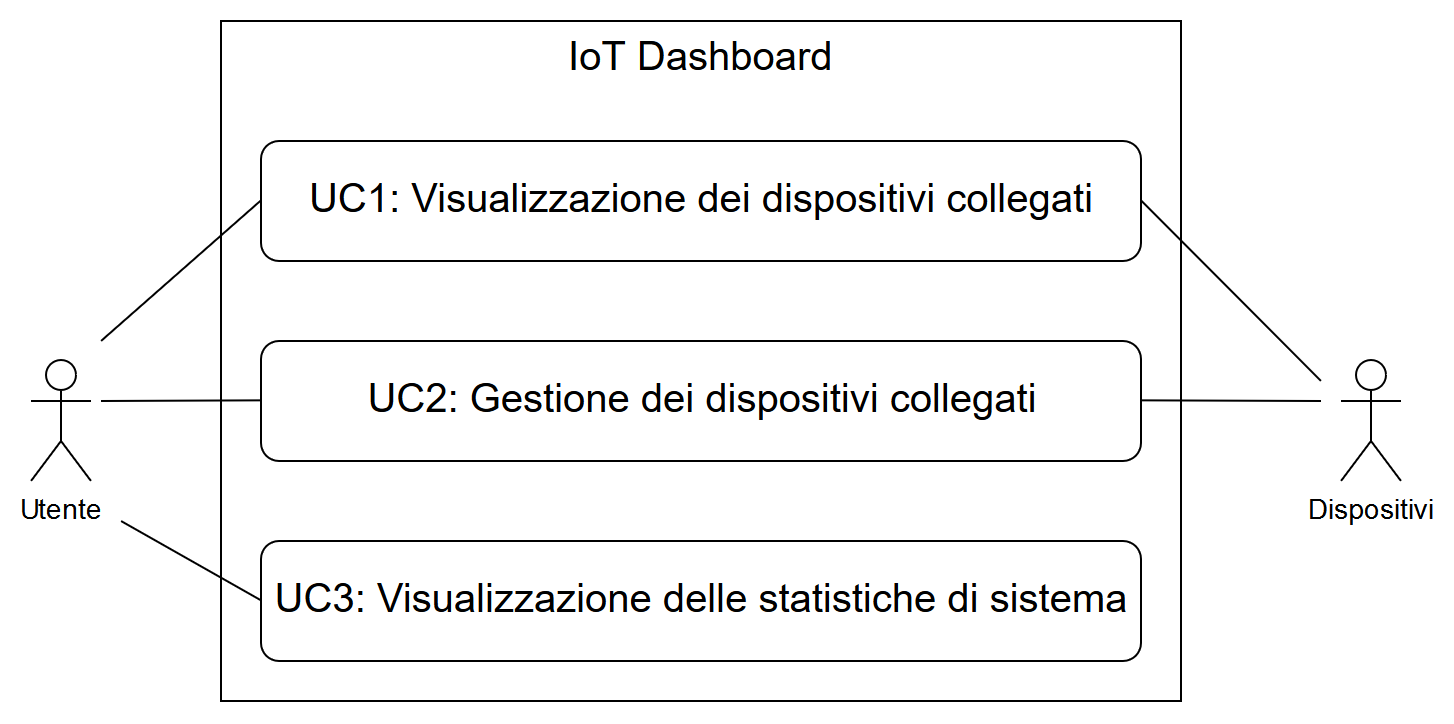
\includegraphics[width=0.9\columnwidth]{usecase/use_cases}
    \caption{Use Case - UC0: Scenario principale}
    \label{fig:scenario-principale}
\end{figure}
% fine uc

Durante le attività di analisi, ho utilizzato la tecnica del \emph{top down} a partire dallo scenario principale menzionato precedentemente per raggiungere, attraverso iterazioni in cui ho raffinato i problemi in sottoproblemi più specifici, uno stato in cui mi è risultato chiaro quali requisiti dovesse soddisfare il prototipo.
Per non allungare eccessivamente questa sezione, riporto l'analisi di uno dei casi d'uso sviluppati: la visualizzazione dei dispositivi collegati al sistema.
La visualizzazione dei dispositivi collegati, caso d'uso UC1 descritto testualmente in ~\ref{uc:uc1} e illustrato utilizzando il linguaggio UML in figura ~\ref{fig:uc1}, mette in relazione l'utente con i dispositivi collegati al sistema. Lo scopo di questa interazione è far conoscere all'utente alcune informazioni elementari riguardanti i dispositivi collegati. In questo caso d'uso ho incluso un'insieme di funzionalità che non cambiano lo scopo del caso d'uso, bensì specificano eventuali interazioni che l'utente può avviare con il sistema. Una delle particolarità del caso d'uso UC1 riguarda il modo con cui ho gestito l'interazione dell'utente con un singolo dispositivo (UC1.3): se l'utente interagisce con un singolo dispositivo nell'ambito di questo caso d'uso, allora l'utente desidera conoscere le informazioni che riguardano quel dispositivo in maggiore dettaglio. Dal momento che le informazioni presentate all'utente in questo \emph{step} riguardano i dispositivi collegati, allora significa che il dispositivo attore in UC1.3 è incluso nella lista dei dispositivi collegati. Da questo pensiero nasce la relazione di inclusione tra l'attore "Dispositivo" e l'attore più esteso "Dispositivi".

% uc testuale
\begin{usecase}{1}{Visualizzazione dei dispositivi collegati}
\usecaseactors{Utente, Dispositivi}
\usecasepre{L'utente ha scelto di visualizzare tutti i dispositivi collegati}
\usecasedesc{L'utente interroga la \emph{dashboard} per conoscere lo stato dei dispositivi collegati}
\usecasepost{L'utente conosce lo stato di tutti i dispositivi collegati al sistema}
\label{uc:uc1}
\end{usecase}

% uc figura
\begin{figure}[!h]
    \centering
    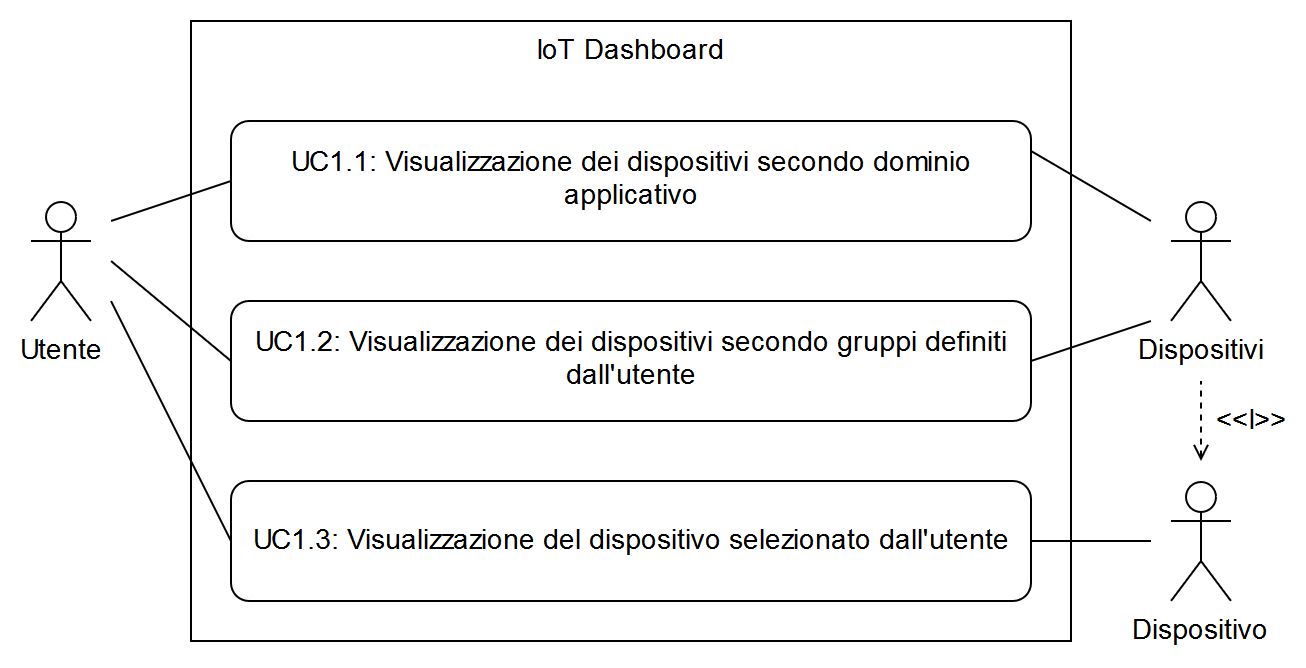
\includegraphics[width=0.9\columnwidth]{usecase/UC1}
    \caption{Use Case - UC1: Visualizzazione dei dispositivi collegati}
    \label{fig:uc1}
\end{figure}
% fine uc

% ## Requisiti
Presento di seguito i requisiti emersi durante l’analisi dei casi d’uso.
Per permetterne una consultazione agevole, ho deciso di inserire i requisiti in un insieme di tabelle dei requisiti suddivise in base alla categoria degli stessi.
In tutte le tabelle cui presenti presento i requisiti indicando:
\begin{itemize}
	\item Identificativo (secondo le regole indicate successivamente);
	\item Categoria di appartenenza fra:
	\begin{itemize}
		\item Obbligatorio, per i requisiti irrinunciabili;
		\item Desiderabile, per i requisiti non strettamente necessari ma che offrono un
    valore aggiunto riconoscibile;
		\item Opzionale, per i requisiti relativamente utili o contrattabili in seguito.
	\end{itemize}
	\item Descrizione esaustiva del requisito;
\end{itemize}
\smallskip

\newenvironment{conditions}
  {\par\vspace{\abovedisplayskip}\noindent\begin{tabular}{>{$}l<{$} @{${}={}$} l}}
  {\end{tabular}\par\vspace{\belowdisplayskip}}

% ### Catalogazione requisiti
Ho scelto di identificare i requisiti seguendo la forma seguente:

\begin{figure}[H]
  \centering
  \[ R[Categoria][Tipo][numero] \]
	dove
	\begin{conditions}
    R & specifica che si tratta di un requisito\\
    Categoria & indica se si tratta di un requisito tra quelli definiti in tabella ~\ref{tab:categoria-requisiti}\\
    Tipo & indica la tipologia del requisito tra quelli definiti in tabella ~\ref{tab:tipi-requisiti}\\
		Numero & è assoluto e rappresenta un riferimento univoco al requisito in questione\\
	\end{conditions}
\end{figure}

Per abbreviare le categorie utilizzate per identificare i requisiti ho associato nella tabella ~\ref{tab:categoria-requisiti} un identificativo a ciascuna categoria.

\begin{table}[H]
\caption{Tabella recante le categorie dei requisiti}
\label{tab:categoria-requisiti}
\begin{tabularx}{\linewidth}{|c|X|}
\hline
\textbf{Identificativo} & \textbf{Descrizione e origine} \\
\hline
M & Obbligatorio (\emph{mandatory}) \\
\hline
A & Desiderabile ((\emph{advisable}) \\
\hline
O & Opzionale (\emph{optional}) \\
\hline
\end{tabularx}
\end{table}

Nella tabella ~\ref{tab:tipi-requisiti} presento i tipi dei requisiti: il tipo indica l'origine del requisito e specifica se il requisito soddisfa una richiesta dell'utente del sistema oppure se esso deriva da una caratteristica del sistema.

\begin{table}[H]
\caption{Tabella recante i tipi dei requisiti}
\label{tab:tipi-requisiti}
\begin{tabularx}{\linewidth}{|c|X|}
\hline
\textbf{Identificativo} & \textbf{Descrizione e origine} \\
\hline
O & Di vincolo (\emph{obligation}) \\
\hline
F & Funzionale (\emph{functional}) \\
\hline
Q & Di qualità (\emph{quality}) \\
\hline
\end{tabularx}
\end{table}

% ### Tabella dei requisiti

% #### Tabella dei requisiti di vincolo
In tabella ~\ref{tab:requisiti-vincolo} indico i requisiti di vincolo che ho individuato durante le attività di analisi dei requisiti. Con questi requisiti indico i vincoli, tecnologici e non, che il sistema deve soddisfare al fine di realizzare un sistema efficiente nella sua implementazione\footnote{Con la locuzione efficienza nell'implementazione mi riferisco alla quantità di risorse spese per soddisfare i requisiti funzionali del sistema (ad es. quantità di tempo investito per l'implementazione delle funzionalità \emph{software}) rispetto al totale delle risorse allocate.}, nel funzionamento e nella manutenzione.

\begin{table}[H]
\caption{Tabella dei requisiti di vincolo}
\label{tab:requisiti-vincolo}
\begin{tabularx}{\linewidth}{|c|c|X|}
\hline
\textbf{Identificativo} & \textbf{Categoria} & \textbf{Descrizione} \\
\hline
RMO1 & Obbligatorio & Il sistema deve essere progettato secondo lo stile di progettazione a microservizi. \\
\hline
RAO2 & Desiderabile & Il sistema può essere implementato utilizzando il linguaggio JavaScript secondo lo standard ECMAScript 2017. \\
\hline
RAO3 & Desiderabile & Il sistema può essere implementato utilizzando il \emph{framework} Node.js per il \emph{backend} e React per il \emph{frontend}. \\
\hline
RMO4 & Obbligatorio & Il sistema deve utilizzare il protocollo MQTT. \\
\hline
\end{tabularx}
\end{table}

% #### Tabella dei requisiti funzionali
In tabella ~\ref{tab:requisiti-funzionali} indico i requisiti funzionali che ho individuato durante le attività di analisi dei requisiti. Con questi requisiti indico le funzionalità che il sistema deve offrire all'utente dello stesso e le classifico in base all'importanza che esse possono avere per l'utente che interagisce con il sistema.

\begin{table}[H]
\caption{Tabella dei requisiti funzionali}
\label{tab:requisiti-funzionali}
\begin{tabularx}{\linewidth}{|c|c|X|}
\hline
\textbf{Identificativo} & \textbf{Categoria} & \textbf{Descrizione} \\
\hline
RMF1 & Obbligatorio & L'utente deve poter visualizzare tutti i dispositivi collegati al sistema. \\
\hline
RMF2 & Obbligatorio & L'utente deve poter visualizzare i dispositivi collegati secondo dominio applicativo. \\
\hline
RAF3 & Desiderabile & L'utente può visualizzare i dispositivi collegati secondo gruppi personalizzati. \\
\hline
RMF4 & Obbligatorio & L'utente deve poter selezionare uno dei dispositivi collegati per visualizzarne le informazioni. \\
\hline
RAF5 & Desiderabile & L'utente può creare un gruppo di dispositivi personalizzato. \\
\hline
RAF6 & Desiderabile & L'utente può modificare uno dei gruppi personalizzati esistenti. \\
\hline
RAF7 & Desiderabile & L'utente può rimuovere uno dei gruppi di dispositivi personalizzati esistenti. \\
\hline
RMF8 & Obbligatorio & L'utente deve poter visualizzare le operazioni messe a disposizione dal dispositivo selezionato. \\
\hline
RMF9 & Obbligatorio & L'utente deve poter selezionare una delle operazioni disponibili. \\
\hline
RMF10 & Obbligatorio & L'utente deve poter visualizzare le statistiche di utilizzo del sistema sistema. \\
\hline
\end{tabularx}
\end{table}

% #### Tabella dei requisiti di qualità
In tabella ~\ref{tab:requisiti-qualita} indico i requisiti di qualità che ho individuato durante le attività di analisi dei requisiti. Con questi requisiti indico le caratteristiche che un sistema \emph{software} deve soddisfare per essere definito \emph{software} di qualità. Nel corso di Ingerneria del Software\footcite{swe-req-qual} ho studiato che i parametri con cui si può misurare la qualità di un \emph{software} possono essere suddivisi in due categorie:
\begin{itemize}
  \item i parametri esterni si riferiscono alla qualità del \emph{software} percepita dagli utenti (correttezza, affidabilità, efficienza, ecc.);
  \item i parametri interni si riferiscono alla qualità del \emph{software} percepita dagli autori del sistema e dai suoi manutentori (manutenibilità, riusabilità, leggibilità, ecc.).
\end{itemize}

\raggedbottom
\begin{table}[htbp]
\caption{Tabella dei requisiti di qualità}
\label{tab:requisiti-qualita}
\begin{tabularx}{\linewidth}{|c|c|>{\setlength\hsize{\hsize}}X|}
\hline
\textbf{Identificativo} & \textbf{Categoria} & \textbf{Descrizione} \\
\hline
ROQ1 & Opzionale & Il sistema deve essere testato, raggiungendo i seguenti obiettivi:
\begin{itemize}
	\item \emph{statement coverage} > 80 \%
	\item \emph{branch coverage} > 90 \%
\end{itemize}\\
\hline
\end{tabularx}
\end{table}

In tabella ~\ref{tab:requisiti-riepilogo} riepilogo i requisiti individuati in sede di analisi, suddividendoli in base al tipo e alla loro categoria d'importanza.

\begin{table}[htbp]
\caption{Tabella di riepilogo dei requisiti}
\label{tab:requisiti-riepilogo}
\begin{tabularx}{\linewidth}{|X|c|c|c|}
\hline
\textbf{Tipo} & \textbf{Obbligatorio} & \textbf{Opzionale} & \textbf{Desiderabile} \\
\hline
Funzionale & 6 & 0 & 4 \\
\hline
Qualitativo & 0 & 1 & 0 \\
\hline
Di vincolo & 2 & 0 & 2 \\
\hline
Totale & 8 & 1 & 6 \\
\hline
\end{tabularx}
\end{table}

\pagebreak

%**************************************************************
\section{Progettazione}
\label{progettazione}

% ### Scopo del documento

In questa sezione del documento definisco la progettazione dell'architettura ad alto livello del progetto di stage.
La sezione include la descrizione dell'architettura del sistema e delle relative componenti \emph{software} e i Design Pattern utilizzati per la progettazione.

L'architettura scelta per il sistema segue lo stile architetturale a microservizi con l'obiettivo di approfondire questo stile architetturale e implementarlo in uno scenario plausibile.
Lo stile architetturale a microservizi descrive un metodo di progettazione delle applicazioni come insiemi di servizi eseguibili indipendentemente, che comunicano tra loro grazie a meccanismi di comunicazione leggeri.
Nel mio caso, la comunicazione tra dispositivi avviene per mezzo del protocollo MQTT. Il protocollo MQTT si basa sul principio che ogni \emph{client} pubblica messaggi, i quali hanno uno o più argomenti, nel gergo tecnico \emph{topic}.
Ogni \emph{client} può registrarsi a determinati argomenti per ricevere tutti i messaggi che altri \emph{client} pubblicano per quell'argomento. Molti \emph{client} si connettono a un \gls{broker} che funziona da intermediario, ricevendo i messaggi pubblicati e inoltrandoli a tutti i \emph{client} sottoscritti ai rispettivi argomenti.
Gli argomenti in MQTT sono trattati gerarchicamente. Questo permette la creazione di argomenti e sottoargomenti, simili alla struttura ad albero di un \emph{filesystem}.
MQTT definisce 3 livelli di qualità della comunicazione in base a quanto \emph{broker} e \emph{client} si impegneranno a ricevere un messaggio.
I \emph{client} decidono il livello massimo di \gls{QoS} che riceveranno.
La scala della QoS definisce i livelli 0, 1 e 2 con affidabilità crescente ma minori performance:
\begin{itemize}
	\item [0]: \emph{broker} e/o \emph{client} invieranno il messaggio al massimo una volta senza richiesta di conferma. A questo livello i messaggi vengono persi se una delle parti si disconnette;
	\item [1]: \emph{broker} e/o \emph{client} invieranno il messaggio almeno una volta con la richiesta di conferma;
	\item [2]: \emph{broker} e/o \emph{client} invieranno il messaggio una sola volta effettuando una trasmissione in 4 step.
\end{itemize}

Per esempio, se un messaggio è pubblicato con QoS 2 e il \emph{client} è sottoscritto all'argomento con QoS 0, il \emph{client} riceverà quel messaggio con QoS 0 (niente richieste di conferma, ecc).
Se un altro \emph{client} è sottoscritto allo stesso argomento con QoS 2 allora riceverà il messaggio con QoS 2 (\gls{handshake} in 4 step).
Alla connessione il \emph{client} imposta un parametro logico che rappresenta una "sessione pulita" in base a come il \emph{client} ritiene affidabile la connessione (`false` indica una connessione affidabile). Se il \emph{client} si disconnette, in tutte le sottoscrizioni con QoS 1 o QoS 2 i messaggi verranno salvati e inviati alla prossima riconnessione del \emph{client}.

Ho progettato le componenti del sistema seguendo il paradigma orientato agli oggetti: in questo modo ho potuto organizzare il codice in moduli riutilizzabili dalle diverse componenti del \emph{software}, diminuendo la possibilità che implementi funzionalità comuni in moduli diversi e con comportamento diverso che potrebbe causare malfunzionamenti nel sistema.
Le attività di progettazione ad alto livello del sistema hanno richiesto da parte mia la redazione di un documento di Specifica Tecnica del sistema, nel quale ho indicato:
\begin{itemize}
  \item le tecnologie e gli strumenti utilizzati;
  \item una panoramica dell'architettura del sistema;
  \item gli approfondimenti riguardanti le componenti definite all'interno dei servizi che compongono il sistema;
  \item i Design Pattern utilizzati all'interno delle componenti dei servizi del sistema.
\end{itemize}

Durante la progettazione delle componenti del prototipo ho utilizzato i diagrammi UML delle classi per rappresentare i tipi delle entità ed evidenziare le relazioni tra queste: in questo modo ho individuato le dipendenze tra le entità e sono quindi stato in grado di modularizzare alcune funzionalità in componenti isolate e riutilizzabili.
Per snellire la procedura di inserimento della specifica delle classi all'interno della Specifica Tecnica ho utilizzato \emph{template}.

Nell'immagine ~\ref{img:overview-arch} illustro la panoramica delle componenti di cui è composta l'architettura utilizzando la notazione dei diagrammi delle componenti UML.

\begin{figure}[H]
    \centering
    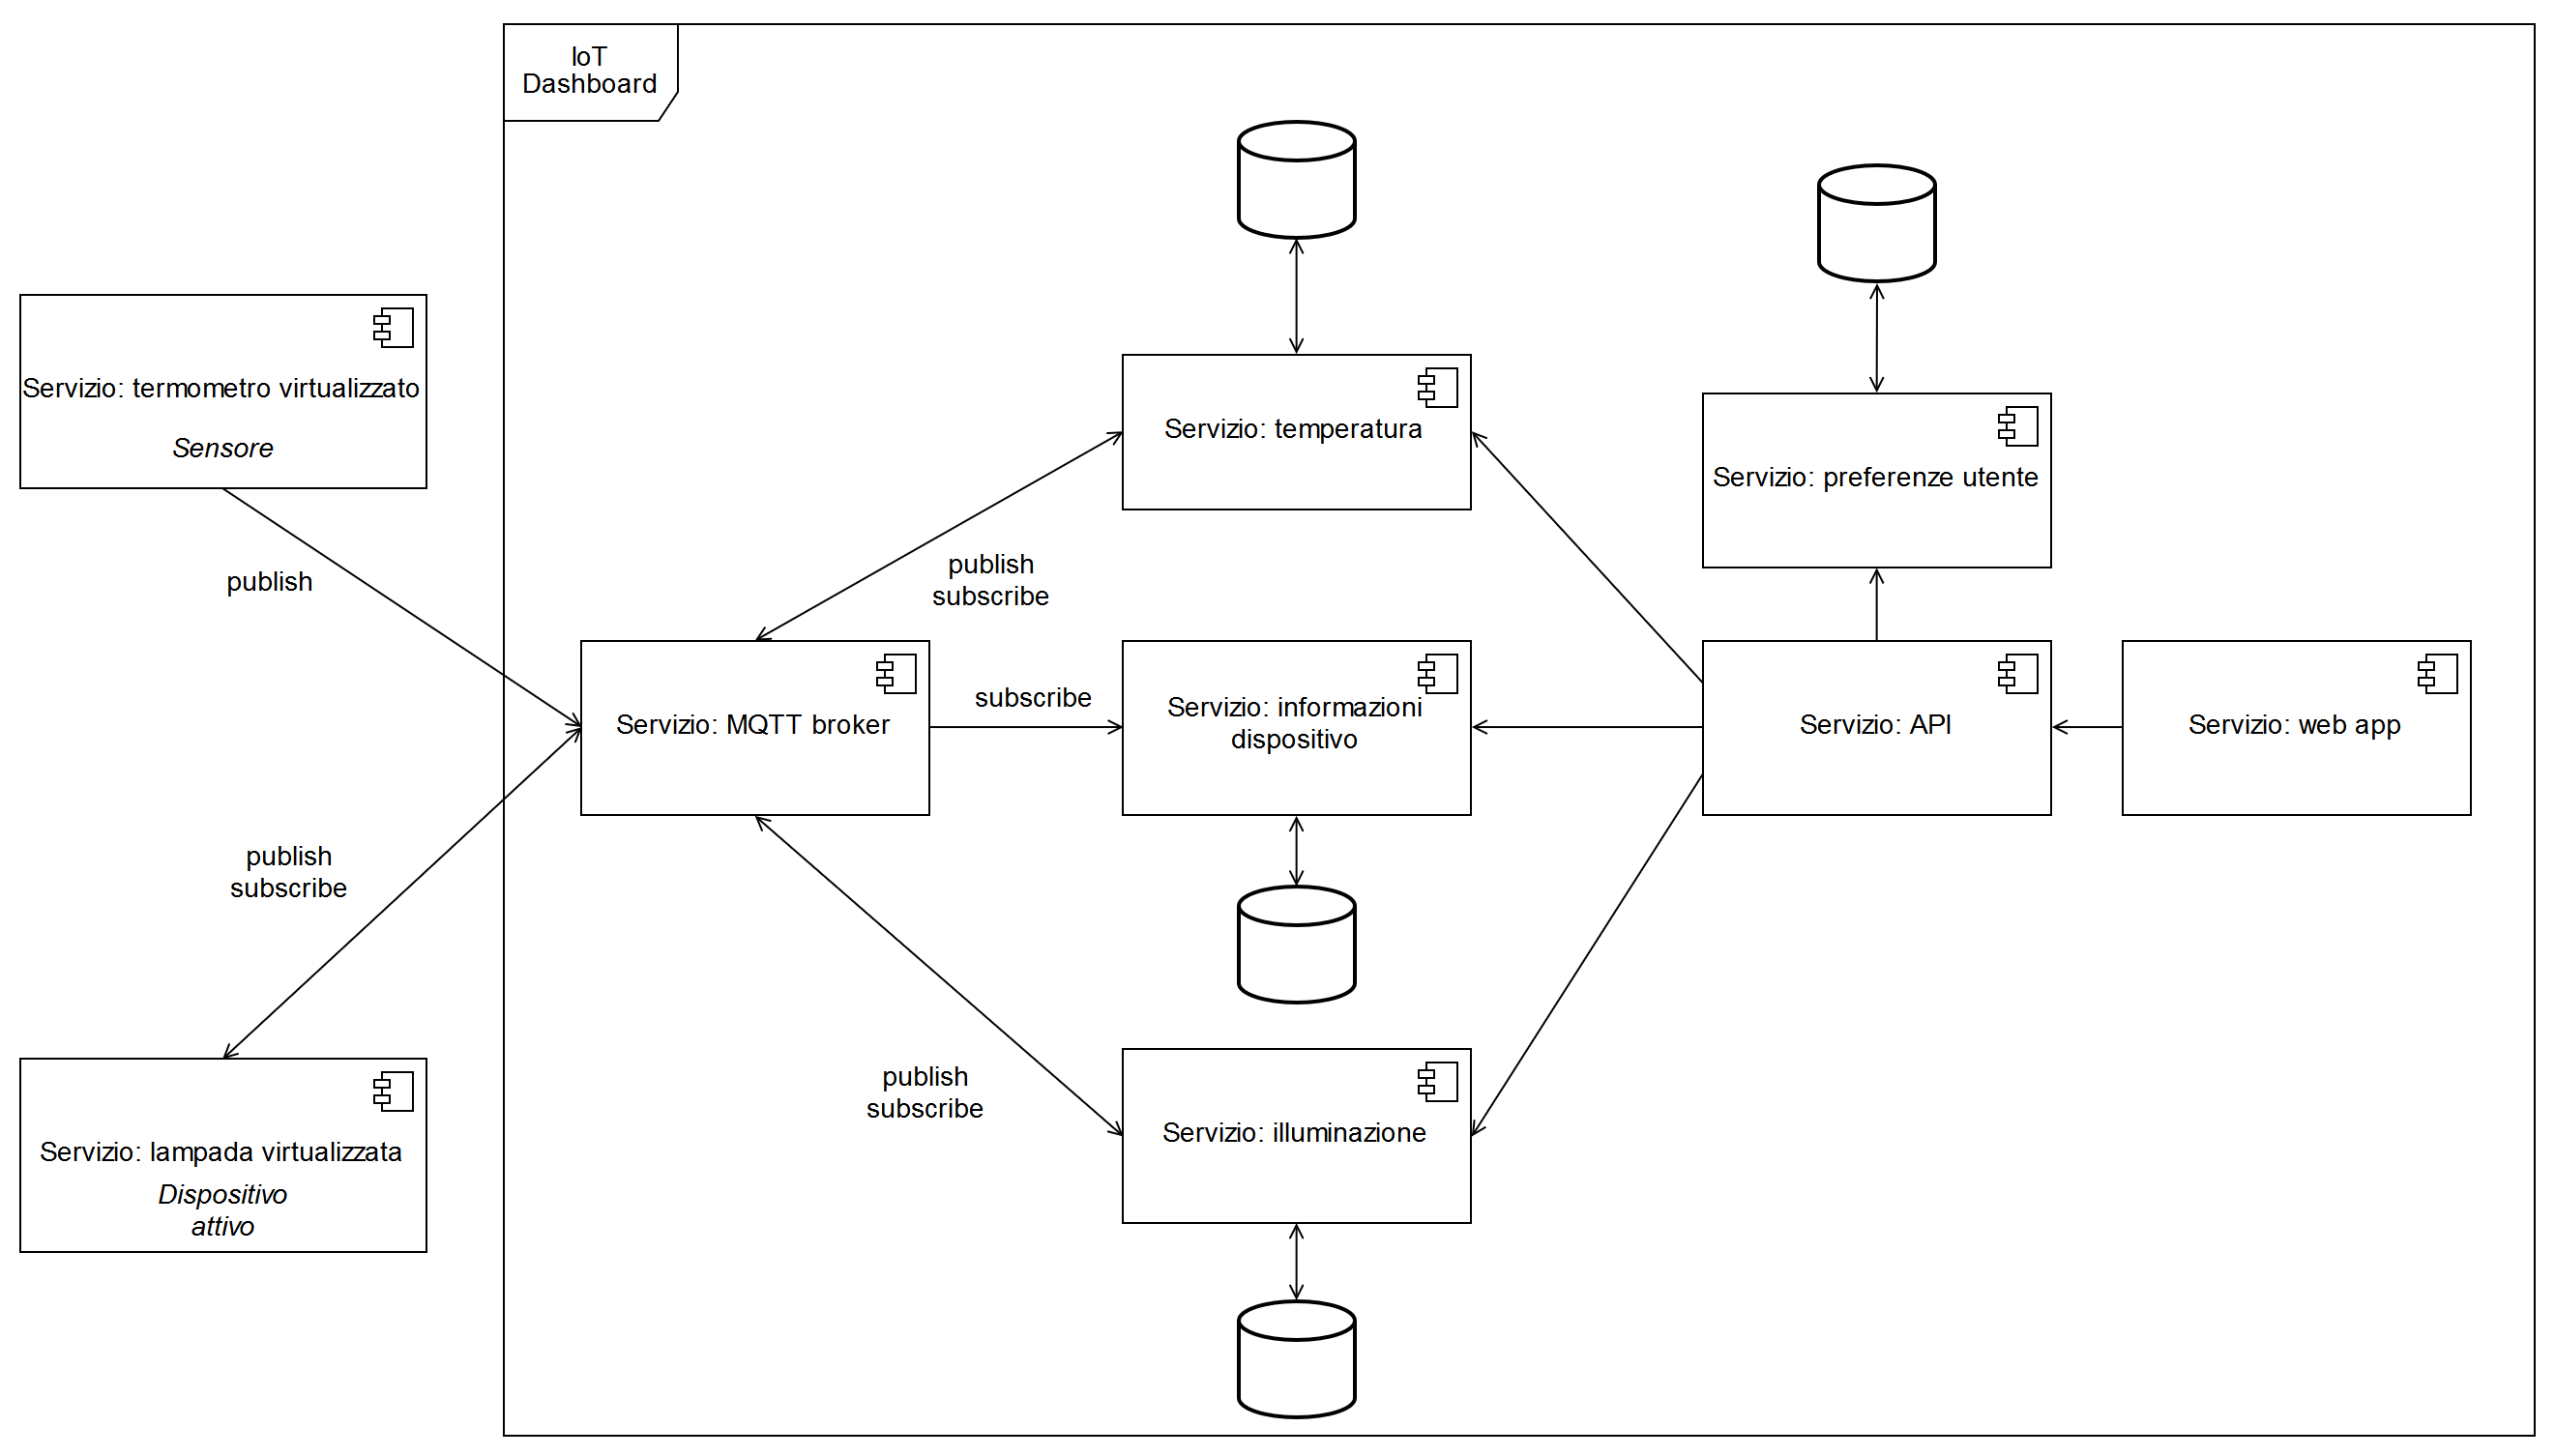
\includegraphics[width=\columnwidth]{progettazione/arch-overview}
    \caption{Panoramica dell'architettura ad alto livello progettata per il prototipo}
    \label{img:overview-arch}
\end{figure}

% ### Servizio: MQTT \emph{broker}
Il \emph{broker} MQTT è il servizio responsabile alla ricezione di tutti i messaggi, alla loro catalogazione e all'invio delle notifiche verso i \emph{client} sottoscritti a ciascuna categoria.
Il \emph{broker} memorizza lo stato di tutti i \emph{client} a lui connessi, inclusi i messaggi non ancora inviati o il cui invio è fallito.

% ### Servizio: termometro _virtualizzato_
Il termometro "virtualizzato" è il servizio responsabile della simulazione di un sensore che invii dati sulla temperatura dell'ambiente in cui si trova.
Esso pubblica periodicamente la temperatura rilevata secondo l'argomento \emph{temperature}, mentre invia secondo l'argomento \emph{hw\_info} i propri dati identificativi, quali produttore, modello, ecc..
Data la relativa importanza i dati vengono inviati con un QoS di livello 0 nella categoria \emph{temperature}, mentre con QoS di livello 1 nella categoria \emph{hw\_info}.
In questo modo al collegamento del dispositivo "virtualizzato" viene effettuato almeno un tentativo di trasmissione delle informazioni relative alle specifiche del dispositivo.
Anche se nel diagramma è disegnato individualmente, è possibile che ve ne siano molteplici.
Nel diagramma ~\ref{fig:classi-termometro} ho illustrato il diagramma delle classi UML a cui sono giunto durante le attività di progettazione ad alto livello. Vista la necessità di generare dati riguardanti la temperatura in maniera psuedocasuale, ho utilizzato il Design Pattern \gls{abstract-factory} per permettere la creazione di funzioni per la generazione della temperatura. Queste funzioni per la generazione della temperatura sono incapsulate in una classe \texttt{TemperatureCurve}, il cui scopo è definire la funzione matematica che restituisce la temperatura in base alla data e ora specificata. L'implementazione di \texttt{TemperatureCurve} progettata per il termometro virtualizzato è \texttt{SineTemperatureCurve}, nella quale restituisco la temperatura sulla base di una temperatura di base specificata e applicando a tale temperatura una funzione sinusoidale.
Ho applicato il Design Pattern Abstract Factory definendo una classe \texttt{TemperatureCurveFactory}, il cui unico scopo è creare oggetti che implementino \texttt{TemperatureCurve}.
Nella tabella ~\ref{tab:classi-termometro} ho elencato le classi sviluppate per soddisfare i requisiti di funzionamento del dispositivo.

\begin{figure}[!h]
    \centering
    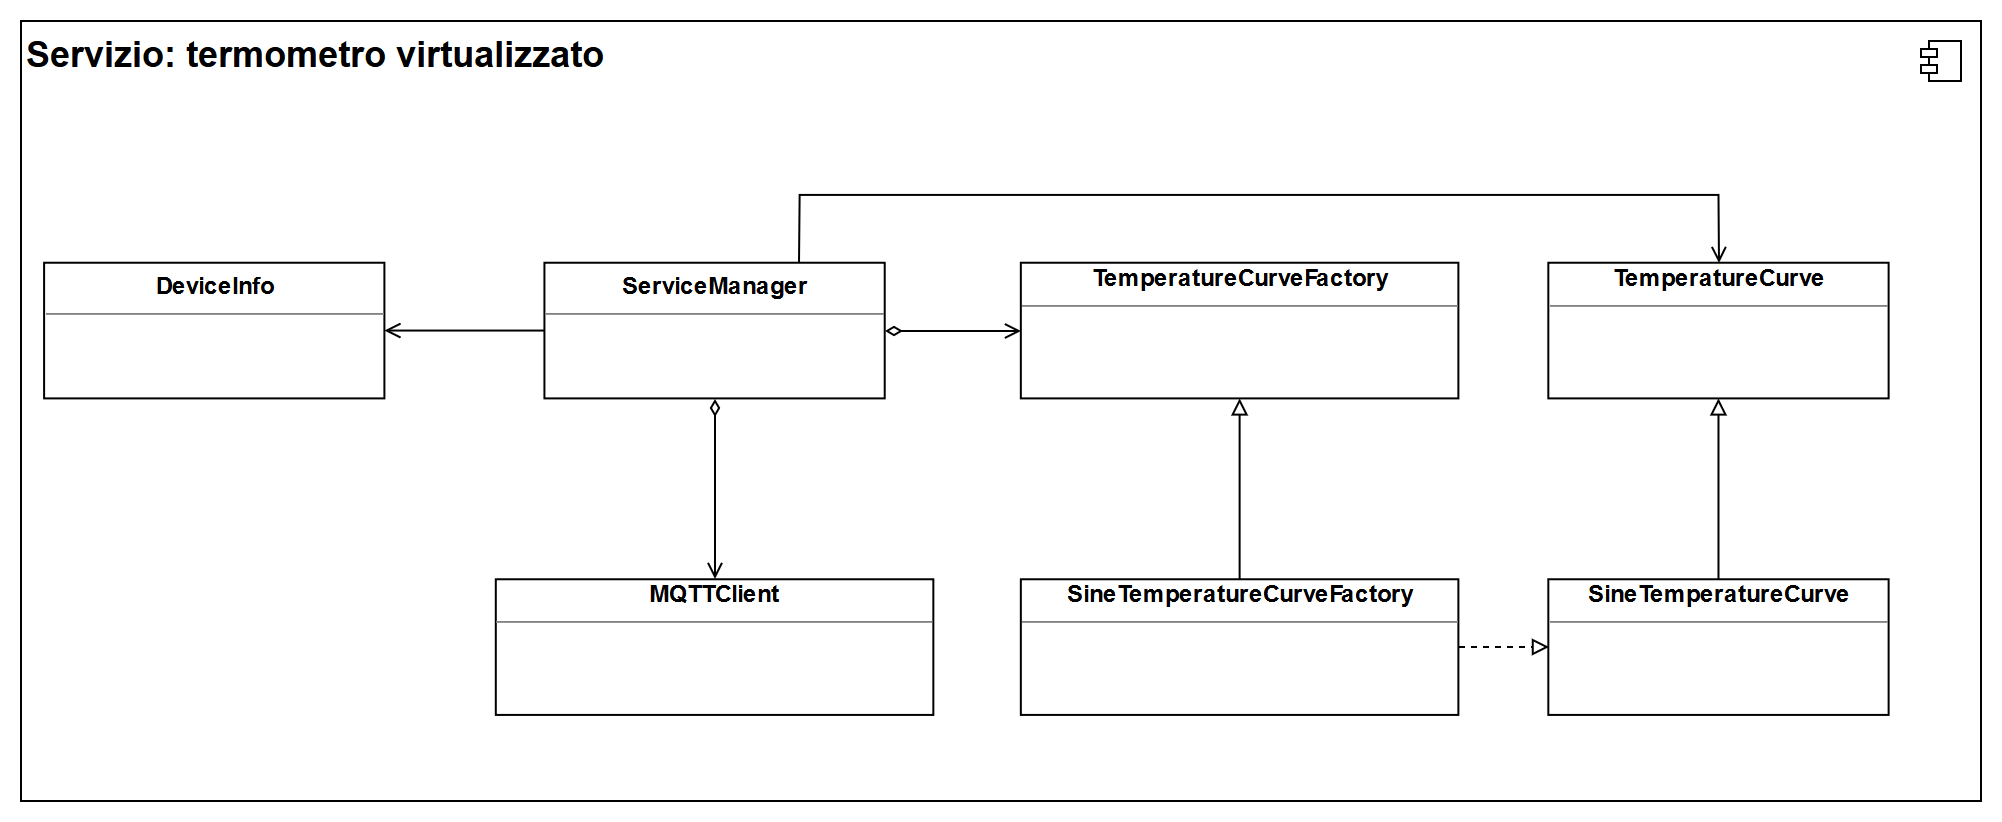
\includegraphics[width=\columnwidth]{progettazione/virtual_temp_sensor_classes}
    \caption{Architettura ad alto livello progettata per il termometro virtualizzato}
    \label{fig:classi-termometro}
\end{figure}

\begin{table}[!h]
\caption{Panoramica delle classi del servizio di simulazione del termometro}
\label{tab:classi-termometro}
\begin{tabularx}{\linewidth}{|c|X|}
\hline
\textbf{Classe} & \textbf{Funzionalità} \\
\hline
\texttt{DeviceInfo} & Classe che indica le informazioni del dispositivo (produttore, modello, revisione, ecc.) pubblicate nel \emph{topic} \emph{hw\_info}.\\
\hline
\texttt{ServiceManager} & Classe responsabile dell'integrazione tra generazione dei dati di temperatura, gestione delle informazioni del dispositivo e invio delle informazioni tramite protocollo MQTT. \\
\hline
\texttt{MQTTClient} & Classe utile all'inizializzazione del \emph{client} MQTT. \\
\hline
\texttt{TemperatureCurveFactory} & Classe Factory che espone la funzionalità di creazione della curva di temperatura, rappresentata dalla classe \texttt{TemperatureCurve}. \\
\hline
\texttt{SineTemperatureCurveFactory} & Implementazione della factory \texttt{TemperatureCurveFactory} per la creazione di oggetti \texttt{SineTemperatureCurve}. \\
\hline
\texttt{TemperatureCurve} & Classe che espone le funzionalità di creazione di una funzione, di aggiunta di rumore pseudocasuale nella funzione creata e di simulazione della temperatura data l'ora corrente. \\
\hline
\texttt{SineTemperatureCurve} & Classe che implementa \texttt{TemperatureCurve} definendo una funzione di simulazione sinusoidale parametrizzabile in ampiezza, frequenza e fase. \\
\hline
\end{tabularx}
\end{table}

% ### Servizio: temperatura
Il servizio relativo alla temperatura si occupa di raccogliere tutti i dati provenienti dai sensori di temperatura, memorizzandoli e mettendoli a disposizione in un formato strutturato per gli altri servizi del sistema.
Il servizio si sottoscrive alla categoria \emph{temperature} e comunica con un QoS di livello 0, inoltre può pubblicare messaggi con la sottocategoria \emph{temperature/active} per usufruire delle funzionalità aggiuntive presenti in dispositivi attivi legati alla temperatura, con un QoS di livello 1.

% Lampada virtualizzata
Con il servizio della lampada "virtualizzata" simulo la presenza nella rete di un dispositivo "attivo": una lampada in grado di comunicare il proprio assorbimento energetico e che è controllabile da remoto.
La lista delle operazioni disponibili è la seguente:
\begin{itemize}
	\item accensione della lampada (QoS di livello 2);
	\item spegnimento della lampada (QoS di livello 2);
	\item richiesta assorbimento energetico (QoS di livello 0);
\end{itemize}
Le operazioni di accensione e spegnimento della lampada necessitano di una affidabilità più elevata delle altre operazioni per evitare l'invio di richieste di accensione e spegnimento multiple.
L'argomento a cui la lampada si sottoscrive è \emph{light/active} e al primo collegamento la lampada invia i propri dati identificativi, pubblicandoli nella categoria \emph{hw\_info}.

% ### Servizio: illuminazione
Il servizio relativo all'illuminazione si occupa di raccogliere e memorizzare tutti i dati pubblicati dai dispositivi nella categoria \emph{light} e permette il controllo dei dispositivi sottoscritti alla categoria \emph{light/active}.
Questo servizio utilizza trasmissioni con tutti i livelli di QoS definiti nel protocollo MQTT: la comunicazione delle operazioni che l'utente esegue vengono trasmessi con il livello di affidabilità maggiore (Qos livello 2) per avere la garanzia che i dati trasmessi siano arrivati ai dispositivi atomicamente, la trasmissione delle specifiche tecniche del dispositivo vengono inviate con un livello di affidabilità intermedio (QoS livello 1) mentre le misurazioni vengono inviate nel modo più efficiente possibile (QoS livello 0).

% ### Servizio: informazioni dispositivo
Il servizio relativo alle informazioni dei dispositivi si occupa di raccogliere e memorizzare tutti i dati pubblicati secondo l'argomento \emph{hw\_info}; utilizza esclusivamente un livello di QoS pari a 1 per aumentare l'affidabilità del sistema a fronte delle attività di identificazione dei dispositivi collegati.

% ### Servizio: preferenze utente
Il servizio di gestione delle preferenze utente si occupa di salvare informazioni quali ad esempio gruppi personalizzati, unità di misura preferite, ecc.
Il servizio non utilizza il protocollo MQTT in quanto non richiede la comunicazione con i dispositivi connessi alla rete, quindi viene utilizzato solamente dal servizio API.

% ### Servizio: API
Il servizio API svolge un ruolo da intermediario tra il servizio che fornisce l'applicazione \emph{web} e i microservizi che raccolgono i dati dei dispositivi.
Esso interroga i servizi "illuminazione", "temperatura" e "informazioni dispositivo"  definiti dal sistema per fornire una interfaccia unificata ai dati.
Per la progettazione del servizio API ho utlizzato uno dei Design Pattern specifici per le architetture a microservizi, ossia il \emph{Gateway Pattern}.
Ho progettato il servizio API in modo \emph{stateless} grazie alla composizione delle API esposte dagli altri servizi: le chiamate effettuate al servizio API vengono dirottate ai rispettivi servizi e opportunamente decorate con informazioni aggiuntive, utili durante le attività di \emph{debug} del prototipo.

% ### Servizio: web app
Il servizio "\emph{web app}" comprende l'applicazione \emph{web} per la consultazione della \emph{dashboard} e include le componenti sviluppate in React per la costruzione dell'interfaccia grafica della \emph{dashboard} e le classi necessarie alla sua pubblicazione sul \emph{web}.
Per conferire un'elevato grado di riutilizzabilità ai componenti creati ho utilizzato il Design Pattern \gls{dp-composite} (rappresentato in figura ~\ref{fig:composite}): nella progettazione dell'interfaccia ho individuato dapprima componenti elementari che estendono la classe \texttt{React.Component} (ad esempio componenti per visualizzare il testo specificato) e gradualmente ho assemblato componenti più complesse, sempre estensioni della classe \texttt{React.Component} (ad esempio unendo la componente di visualizzazione del testo con la componente di visualizzazione di una immagine). Attraverso questo procedimento \emph{bottom up} ho concluso la progettazione delle componenti dell'interfaccia, giungendo alla componente \texttt{UIPage}, la quale è anch'essa una componente React che specifica quali componenti e con quale struttura visualizzare a schermo una determinata pagina. Ciascuna pagina dell'applicazione \emph{web} è quindi un \emph{collage} di componenti più o meno complesse che mi hanno permesso di riutilizzare i componenti elementari in molte pagine dell'applicazione.

\begin{figure}[H]
    \centering
    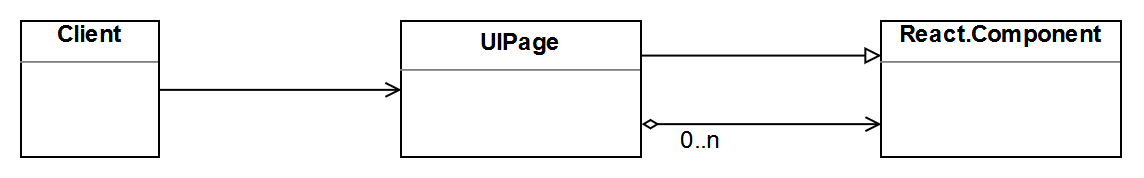
\includegraphics[width=0.95\columnwidth]{progettazione/composite}
    \caption{Rappresentazione semplificata del Design Pattern Composite}
    \label{fig:composite}
\end{figure}

Nel diagramma ~\ref{fig:classi-web} indico l'architettura ad alto livello progettata per il servizio di presentazione delle informazioni e nella tabella ~\ref{tab:classi-web} descrivo le classi sviluppate.

\begin{figure}[H]
    \centering
    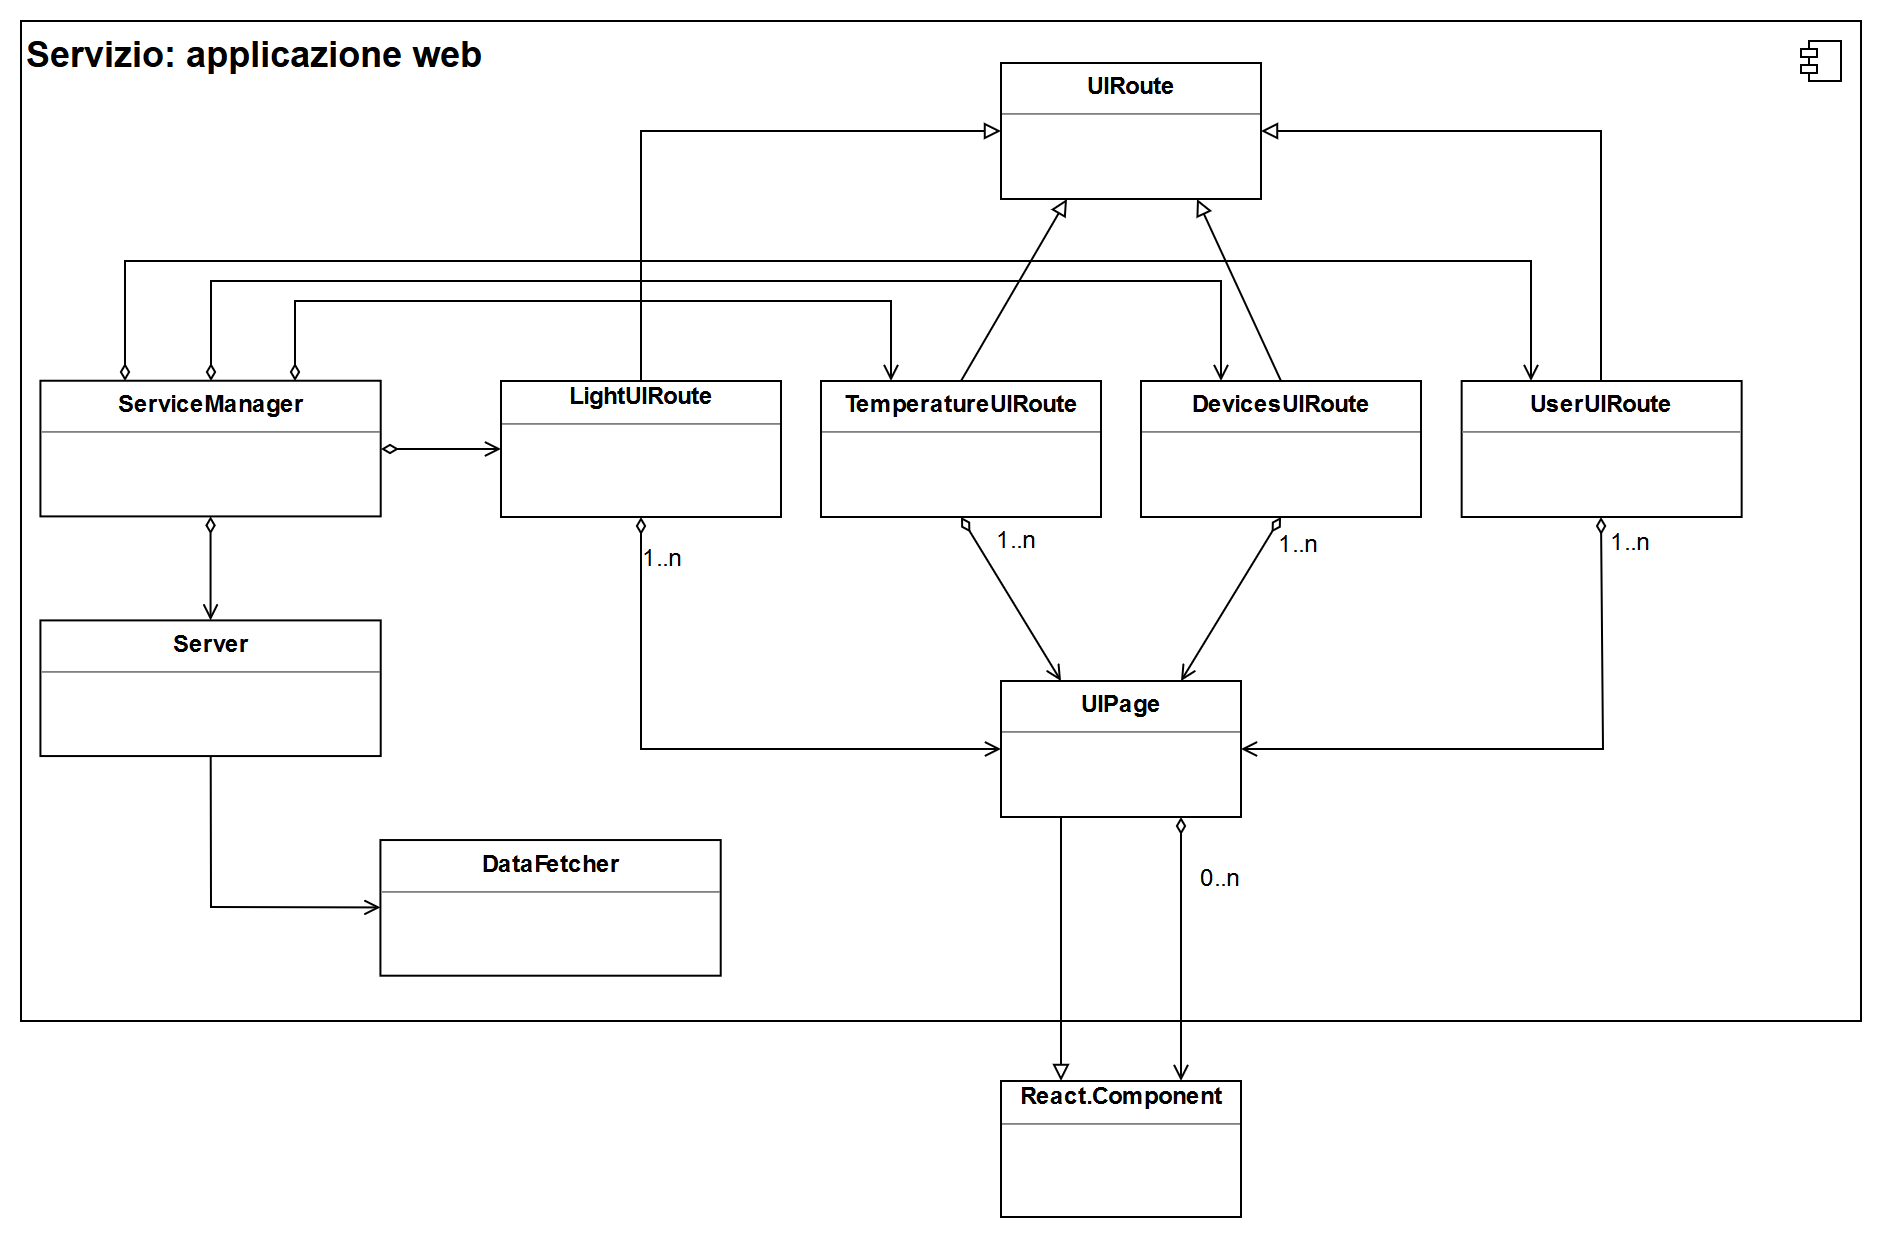
\includegraphics[width=0.90\columnwidth]{progettazione/web_service_classes}
    \caption{Architettura ad alto livello progettata per il servizio \emph{web app}}
    \label{fig:classi-web}
\end{figure}

\begin{table}[htbp]
\caption{Panoramica delle classi del servizio API}
\label{tab:classi-web}
\begin{tabularx}{\linewidth}{|c|X|}
\hline
\textbf{Classe} & \textbf{Funzionalità} \\
\hline
\texttt{ServiceManager} & Classe responsabile dell'integrazione tra istanza del server, pagine esposte e interfaccia di richeista dati. \\
\hline
\texttt{DataFetcher} & Modulo che si occupa di effettuare le richieste al servizio API secondo le definizioni fornite dal servizio. \\
\hline
\texttt{Server} & Classe responsabile del ciclo di vita del server Node.js. Effettua le richieste definite dalle istanze di \texttt{UIRoute} per ricevere i dati, utilizzando un'istanza di \texttt{DataFetcher}. \\
\hline
\texttt{UIRoute} & Interfaccia utilizzata per definire le richieste da effettuare per ricevere le informazioni che popolano le pagine della rotta. \\
\hline
\texttt{UserUIRoute} & Implementazione di \texttt{UIRoute} che definisce le richieste per ottenere o modificare le preferenze dell'utente ed espone le pagine di visualizzazione e modifica delle preferenze utente. \\
\hline
\texttt{DevicesUIRoute} & Implementazione di \texttt{UIRoute} che definisce le richieste per ottenere informazioni sui dispositivi collegati ed espone le pagine di visualizzazione di questi. \\
\hline
\texttt{TemperatureUIRoute} & Implementazione di \texttt{UIRoute} che definisce le richieste per ottenere dati legati alla temperatura, visualizzare ed eseguire operazioni con dispositivi attivi e ne permette la visualizzazione. \\
\hline
\texttt{LightUIRoute} & Implementazione di \texttt{UIRoute} che definisce le richieste per ottenere dati legati all'illuminazione, visualizzare ed eseguire operazioni con dispositivi attivi e ne permette la visualizzazione. \\
\hline
\texttt{UIPage} & Implementazione di un componente React (\texttt{React.Component}) che rappresenta una pagina. La pagina visualizzata può contenere più figli anch'essi componenti React. \\
\hline
\texttt{React.Component} & Classe che rappresenta una componente grafica nel \emph{framework} React. \\
\hline
\end{tabularx}
\end{table}

\pagebreak

%**************************************************************
\section{Implementazione e verifica}

Durante le attività di implementazione delle specifiche del sistema ho scritto, oltre al codice sorgente dei servizi, anche documenti in cui indico le istruzioni per eseguire le singole componenti del sistema e specifico le risorse esposte dalle stesse.
I documenti in cui indico le risorse esposte dai servizi sono rivolti agli utenti più esperti che vogliono approfondire le funzionalità offerte dai servizi. Nelle mie previsioni questi utenti grazie ai documenti di specifica dovrebbero essere in grado di implementare le altre componenti del sistema, sostituendo le componenti da me implementate. Ho scritto questi documenti contestualmente all'implmentazione delle funzionalità nel codice sorgente, adeguandoli manualmente ad ogni modifica compiuta nel codice sorgente.\\
Ho deciso di scrivere i documenti in cui indico le istruzioni per eseguire il progetto sia in lingua italiana, sia in lingua inglese dal momento che il progetto è disponibile pubblicamente su GitHub. Nel farlo ho seguito alcuni consigli che ho tratto dalla lista degli articoli presenti al link \url{https://github.com/matiassingers/awesome-readme\#articles}: in questo \gls{repository} l'autore ha raccolto collegamenti a:
\begin{itemize}
  \item esempi di pagine informative dei rispettivi progetti caratterizzate da una buona struttura e da contenuti adeguati agli utenti a cui questi progetti sono indirizzati;
  \item articoli di autori che espongono la loro opinione riguardo a come dovrebbero essere scritti i documenti che gli utenti devono leggere in sede di esplorazione del progetto;
  \item strumenti che facilitano la scrittura dei documenti informativi.
\end{itemize}
Nelle istruzioni ho incluso i riferimenti per installare i \emph{software} richiesti e ho fatto in modo che i procedimenti da seguire fossero i più brevi possibili (procedimenti con al massimo 5 istruzioni da seguire). Ho scritto queste istruzioni solamente quando mi sono accertato che le componenti fossero abbastanza stabili nel loro funzionamento da poter essere potenzialmente usate da altri utenti.\\
Ho scritto la documentazione del codice sorgente contestualmente al codice sorgente; la documentazione del codice sorgente consiste in commenti nei sorgenti JavaScript in cui spiego:
\begin{itemize}
	\item lo scopo delle proprietà degli oggetti;
	\item il tipo delle proprietà degli oggetti: in questo caso ho preferito annotare il tipo delle proprietà degli oggetti nella documentazione in quanto JavaScript non è staticamente tipizzato e quindi la dichiarazione di variabili non consente di specificare un tipo con cui il compilatore e l'interprete validino il codice sorgente;
	\item gli algoritmi utilizzati per l'implementazione delle funzionalità.
\end{itemize}
Ho scritto i commenti nel codice sorgente, come da \emph{best practice} per i progetti distribuiti pubblicamente, in lingua inglese.

Prima di iniziare le attività di codifica ho utilizzato Yeoman (\url{http://yeoman.io/}) per generare un \emph{template} che ho utilizzato per implmentare tutti i servizi. Nel \emph{template} ho specificato le dipendenze comuni a tutti i servizi e ho configurato la struttura dei progetti in modo che fosse ripetibile per tutti i servizi.
Ogni servizio, grazie alla generazione per mezzo del \emph{template}, ha al suo interno gli strumenti di analisi statica e dinamica del codice, un documento di \emph{README} contenente le informazioni specifiche per il servizio e un \emph{Dockerfile} responsabile della creazione dei \emph{container}.
Lo strumento principale che ho utilizzato durante la codifica è l'\emph{editor} Visual Studio Code, indicato in tabella ~\ref{tab:strumenti}, grazie al quale ho utilizzato gli strumenti di analisi statica e dinamica del codice durante la sua scrittura.

Le attività di verifica garantiscono che l'esecuzione delle attività pianificate nel corso dello svolgimento di un progetto non introducano errori.
Durante le attività di verifica dei requisiti ho controllato la loro consistenza e la loro completezza, accertandomi che fossero chiaramente definiti, tuttavia ho tralasciato il controllo della loro realizzabilità confidando nelle mie capacità implementative.
Durante le attività di progettazione ad alto livello del prototipo ho iterato le attività di verifica sui diagrammi delle classi UML al fine di verificare che essi rispondessero a due criteri:
\begin{itemize}
  \item il grado di accoppiamento medio delle classi, calcolato come differenza in valore assoluto tra le relazioni in ingresso e le relazioni in uscita per ogni classe, sia nell'intervallo [0, 2] (ogni classe può utilizzare in media fino a un massimo di due altre classi);
  \item le classi all'interno di ciascun microservizio offrano le funzionalità essenziali per soddisfare i requisiti correlati e non dipendano dagli altri servizi per funzionare.
\end{itemize}
Ai due criteri ho associato gradi di importanza non equivalenti: ho preferito concentrarmi sul secondo criterio, che ho potuto applicare a tutti i servizi ad eccezione del servizio API intermediario con i \emph{client}) per acquisire esperienza nell'applicazione del concetto \emph{micro} ai servizi richiesto dalle archietture a microservizi.
Ho svolto le attività di verifica durante l'implementazione del \emph{software} da due lati:
\begin{itemize}
  \item ho pianificato il primo insieme di attività del processo di verifica del prodotto utilizzando gli strumenti di analisi statica per prevenire errori comuni e facilmente risolvibili automaticamente;
  \item ho pianificato il secondo insieme di attività del processo di verifica del prodotto effettuando prove durante l'esecuzione del \emph{software}.
\end{itemize}
Ho condotto l'analisi dinamica del prodotto sia con l'ausilio di strumenti di test automatici, sia effettuando prove manuali, simulando l'interazione di un \emph{client}, inteso come attore, con i servizi.
Ho progettato i test per raggiungere la copertura del codice fissata durante l'attività di Analisi dei requisiti (riferimento ~\ref{tab:requisiti-qualita}).
Durante la progettazione dei test ho scelto di approfondire la progettazione dei test d'unità di tutte le componenti progettate come primo \emph{step} mentre ho tralasciato la progettazione dei test d'integrazione dei servizi: ho perseguito questa scelta perché ho ritenuto più importante aumentare l'affidabilità intrinseca di ciascun servizio indipendentemente dagli altri.
Uno dei fattori che mi ha consentito di effetuare questa scelta consiste nell'individualità dell'implementazione del progetto: se al progetto avessero collaborato uno o più sviluppatori, avrebbe assunto maggiore importanza la corretta interazione tra i servizi. Inoltre, dal momento che i servizi che ho progettato hanno un flusso dei dati ben definito, mi ha permesso di tenere allineate le modifiche attraverso i servizi in efficienza.
Nei test ho usato ampiamente \emph{mock} e \emph{stub} per isolare le eventuali dipendenze tra un modulo e un altro all'interno dello stesso servizio. Come avevo previsto durante lo studio degli argomenti, la componente in cui ho avuto alcune difficoltà nell'implementazione dei test consiste nei moduli che dialogano con un \emph{database}: per arginare il problema ho utilizzato librerie accessorie presenti su npm per simulare le risposte che i \emph{database} inviano nel caso in cui si verifichino errori. In questo modo ho potuto testare con successo anche eventuali malfunzionamenti relativi al collegamento con i \emph{database}.
Ho elencato i risultati della copertura del codice raggiunta al termine dello stage nella tabella ~\ref{tab:coverage}.

\begin{table}[H]
\caption{Tabella che specifica la copertura del codice raggiunta per ciascun servizio}
\label{tab:coverage}
\begin{tabularx}{\linewidth}{|X|c|c|}
\hline
\textbf{Servizio} & \textbf{\emph{Statement coverage}} & \textbf{\emph{Branch coverage}} \\
\hline
MQTT Broker & 93 \% & 90 \% \\
\hline
Sensore di temperatura "virtualizzato" & 97 \% & 85 \% \\
\hline
Temperatura & 92 \% & 81 \% \\
\hline
Lampada \emph{smart} "virtualizzata" & 83 \% & 67 \% \\
\hline
Illuminazione & 91 \% & 65 \% \\
\hline
Informazioni dispositivi & 90 \% & 77 \% \\
\hline
Preferenze utente & 90 \% & 79 \% \\
\hline
API & 70 \% & 70 \% \\
\hline
Applicazione \emph{web} & 50 \% & 63 \% \\
\hline
\textbf{Totale} & 85,44 \% & 75,22 \% \\
\hline
\end{tabularx}
\end{table}

%**************************************************************
\section{Validazione dei requisiti}
\label{val-req}

Nella tabella ~\ref{tab:validazione-requisiti}) ho elencato lo stato dell'implementazione dei requisiti citati in Analisi (riferimento ~\ref{ar})).

\begin{table}[H]
\caption{Tabella dei requisiti funzionali}
\label{tab:validazione-requisiti}
\begin{tabularx}{\linewidth}{|c|c|X|}
\hline
\textbf{Identificativo} & \textbf{Categoria} & \textbf{Esito} \\
\hline
RMF1 & Obbligatorio & Soddisfatto \\
\hline
RMF2 & Obbligatorio & Soddisfatto \\
\hline
RAF3 & Desiderabile & Omesso \\
\hline
RMF4 & Obbligatorio & Soddisfatto \\
\hline
RAF5 & Desiderabile & Omesso. \\
\hline
RAF6 & Desiderabile & Omesso. \\
\hline
RAF7 & Desiderabile & Omesso \\
\hline
RMF8 & Obbligatorio & Soddisfatto \\
\hline
RMF9 & Obbligatorio & Soddisfatto \\
\hline
RMF10 & Obbligatorio & Parzialmente soddisfatto \\
\hline
ROQ1 & Opzionale & Soddisfatto \\
\hline
RMO1 & Obbligatorio & Soddisfatto \\
\hline
RAO2 & Desiderabile & Soddisfatto \\
\hline
RAO3 & Desiderabile & Soddisfatto \\
\hline
RMO4 & Obbligatorio & Soddisfatto \\
\hline
\end{tabularx}
\end{table}

Durante lo svolgimento dello stage ho deciso di non implementare i requisiti relativi alla personalizzazione dei gruppi di dispositivi perché ho incontrato alcune difficoltà relative alla composizione dei servizi che hanno rallentato l'implementazione delle funzionalità dei servizi. Come avevo previsto in sede di valutazione dei rischi (riferimento ~\ref{tab:rischi-arch-microservizi}), la difficoltà nel reperimento delle informazioni correlate ad esempi pratici delle architetture a microservizi ha causato un generale rallentamento delle attività di sviluppo.
In particolare, ho avuto difficoltà in due momenti:
\begin{itemize}[nosep]
  \item durante lo sviluppo di una soluzione sperimentale che permettesse di utilizzare la tecnica dello \gls{sharding} tra molteplici \emph{database} in un contesto di utilizzo basato sui \emph{container};
  \item durante lo sviluppo del servizio di integrazione delle API (servizio API citato in ~\ref{progettazione}) fornite dai singoli microservizi.
\end{itemize}
Ho riscontrato la prima problematica a causa della documentazione legata allo \emph{sharding} del \emph{database} considerato: dal momento che essa è indirizzata per installazioni dei \emph{database} direttamente sui calcolatori ho avuto difficoltà a trasportare quelle istruzioni nell'ambito della composizione di \emph{container}, richiedendo una quantità superiore a quella che avevo valutato per essere implementata.\\
Proseguendo con la seconda criticità, questa si è verificata a causa di una mia incomprensione del meccanismo di condivisione della rete nell'ambito dell'orchestrazione dei servizi attraverso Docker Compose: nella pratica i servizi legati alla temperatura, all'illuminazione, alla gestione delle informazioni dei dispositivi e alle preferenze utente potevano essere interrogati individualmente, tuttavia non riuscivano a comunicare con il servizio di integrazione (servizio API) perché Docker Compose internamente isolava i \emph{container} in sottoreti virtuali senza possibilità di comunicare tra loro. Ho risolto il problema definendo manualmente una nuova sottorete virtuale, comune a tutti i servizi, che ha permesso al sistema di funzionare correttamente.\\
Per quanto riguarda il requisito RMF10, relativo alla visualizzazione delle statistiche di sistema, ho deciso di implementare solamente la componente di controllo della salute dei servizi che compongono il sistema \emph{healthcheck}, tralasciando le componenti di integrazione dei dati raccolti dai servizi e le componenti di visualizzazione dei dati citati.\\
A causa dei rallentamenti menzionati ho scelto di non implementare alcune funzionalità perché, sebbene le avessi catalogate come desiderabili, la quantità di risorse rimanenti non sarebbe stata sufficiente alla loro corretta implementazione, quindi ho preferito allocare tempo per migliorare la qualità del \emph{software} sviluppato aumentando la copertura del codice sorgente, implementando un numero maggiore di test di unità. Mi è ora chiaro che alcuni dei requisiti da me classificati avrebbero richiesto ulteriori passaggi di verifica: la fattibilità e la valutazione più attenta del rapporto importanza della funzionalità paragonato alle risorse a disposizione avrebbero evidenziato che alcuni requisiti non erano implementabili nelle ore destinate al progetto di stage.
